\documentclass[]{article}

\usepackage{mathtools,mathrsfs,url,fancyhdr, graphicx,amssymb,amsthm,tensor,listings,float,color}
\usepackage[dvipsnames]{xcolor}
\usepackage{tikz,url,float}
\usetikzlibrary{decorations.pathmorphing}
\usetikzlibrary{decorations.pathmorphing}
\usetikzlibrary{arrows.meta}
\tikzset{>={Latex[width=2mm,length=2mm]}}
\graphicspath{ {images/} }
\newcommand\numberthis{\addtocounter{equation}{1}\tag{\theequation}}

%opening
\title{Introduction into General Relativity\\Assignment 5.1\\Penrose--Carter diagram for an eternally accelerating observer/particle}
\author{Simon Crase}

\begin{document}

\maketitle

\section{Penrose--Carter diagram}

We will use the following parametric form for a steadily accelerating particle: \cite[equation (7)]{akhmedev2016}:
\begin{align*}
t=\sinh(s), x=\cosh(s)-1 \numberthis\label{eq:steadily_accelerating_particle}
\end{align*}
where we have eliminated \emph{a} by an obvious transformation.

From (\ref{eq:steadily_accelerating_particle})
\begin{align*}
	t+x &= \sinh(s) + \cosh(s)-1\\
	&=2e^s-1\\
	t-x &= \sinh(s) - \cosh(s)+1\\
	&=-2e^{-s}+1\\
	&\simeq 1 \text{, for } s \rightarrow \infty \text{, Hence:}\\
	t+x &= \tan(\frac{\psi + \xi}{2}) \text{, \cite[V,2]{akhmedev2016}}\\
	&\simeq\infty \text{, as } s \rightarrow \infty \\
	t-x &= \tan(\frac{\psi - \xi}{2}) \\
	&\simeq 1 \text{, as } s \rightarrow \infty \text{, hence, as }  s \rightarrow \infty \\
	\frac{\psi + \xi}{2} &\simeq \frac{\pi}{2} \land \frac{\psi - \xi}{2} \simeq \frac{\pi}{4} \numberthis\label{eq:asymptote}
\end{align*}

From (\ref{eq:asymptote}), as $s \rightarrow \infty$, $(\psi,\xi) \rightarrow \cal{J}^+$ along an asymptote given by $\psi-\xi=\frac{\pi}{2}$, which is perpendicular to $\cal{J}^+$. Similarly, as $s \rightarrow -\infty$, $(\psi,\xi) \rightarrow \cal{J}^-$ along an asymptote which is perpendicular.

\begin{figure}[H]
	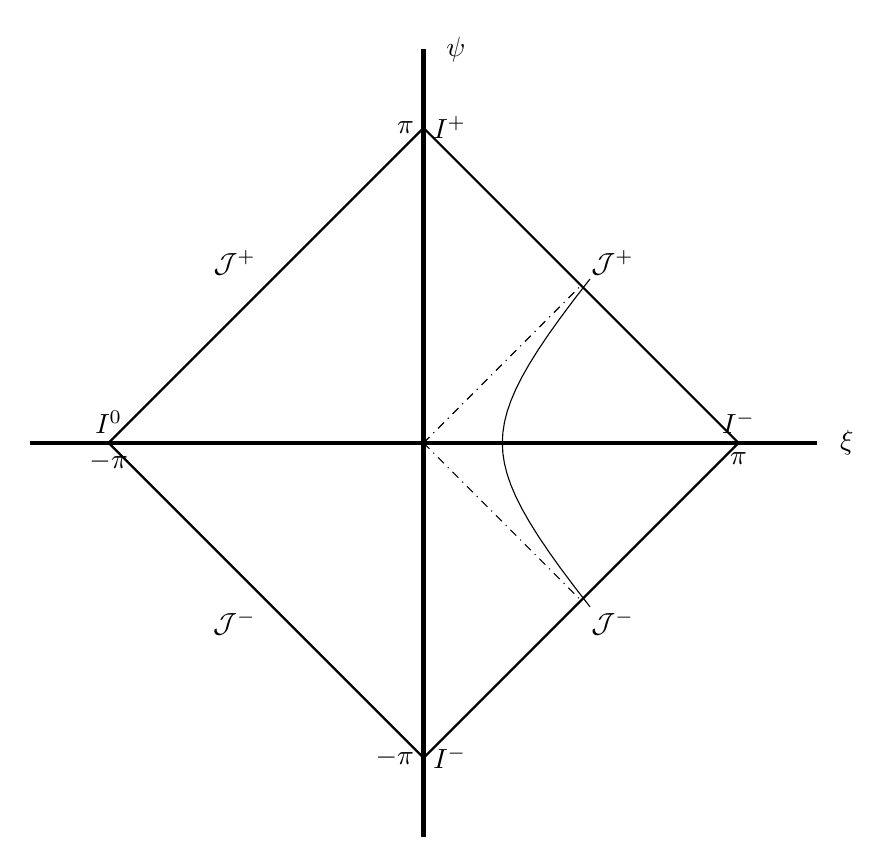
\begin{tikzpicture}
	\draw[black, ultra thick] (0,-5) -- (0,5) node [label=right:{$\psi$}] {};
	\draw[black, ultra thick] (-5,0) -- (5,0) node [label=right:{$\xi$}] {};
	\draw[black,thick] (0,4) -- (4,0) node[midway, above right]    {$\cal{J}^+$};
	\draw[black,thick] (4,0) -- (0,-4) node[midway, below right]    {$\cal{J}^-$};
	\draw[black,thick] (0,-4) -- (-4,0) node[midway, below left]    {$\cal{J}^-$};
	\draw[black,thick] (-4,0) -- (0,4)  node[midway, above left]    {$\cal{J}^+$};
	\filldraw[black] (0,4) circle (0pt) node[anchor=west] {$I^+$};
	\filldraw[black] (0,4) circle (0pt) node[anchor=east] {$\pi$};
	\filldraw[black] (0,-4) circle (0pt) node[anchor=west] {$I^-$};
	\filldraw[black] (0,-4) circle (0pt) node[anchor=east] {$-\pi$};
	\filldraw[black] (-4,0) circle (0pt) node[anchor=south] {$I^0$};
	\filldraw[black] (4,0) circle (0pt) node[anchor=north] {$\pi$};
	\filldraw[black] (4,0) circle (0pt) node[anchor=south] {$I^-$};
	\filldraw[black] (-4,0) circle (0pt) node[anchor=north] {$-\pi$};
	\draw[black,thin, dash dot] (0,0) -- (2,2);
	\draw[black,thin, dash dot] (0,0) -- (2,-2);
	\pgfmathsetmacro{\e}{1.5}   % eccentricity
	\pgfmathsetmacro{\a}{1}
	\pgfmathsetmacro{\b}{(\a*sqrt((\e)^2-1)} 
	\draw plot[domain=-1.38:1.38] ({\a*cosh(\x)},{\b*sinh(\x)});
	\end{tikzpicture}
\end{figure}


\begin{thebibliography}{9}
	
	\bibitem{akhmedev2016}
	Emil T. Akhmedev,
	\emph{Lectures on General Theory of Relativity},
	2016,
	\url{https://arxiv.org/pdf/1601.04996v6.pdf}.

\end{thebibliography}


\end{document}
